\section{Risultati Ottenuti}

\subsubsection*{Grafico senza intervento}
Il seguente grafico \ref{fig:abm_no_intervent} mostra l'andamento delle curve del modello
quando questo viene eseguito senza alcuna tipologia di intervento. Questo andamento tuttavia e' mostrato 
in maniera cumulativa rispetto all'andamento dei singoli agenti, il quale puo' avere comportamentei 
differenti in base a se appare o meno una variante, come specificato in figura \ref{fig:voc}, oppure 
dipendentemente dal tipo di contromisure applicate. 

\begin{minipage}{\linewidth}
	\centering
	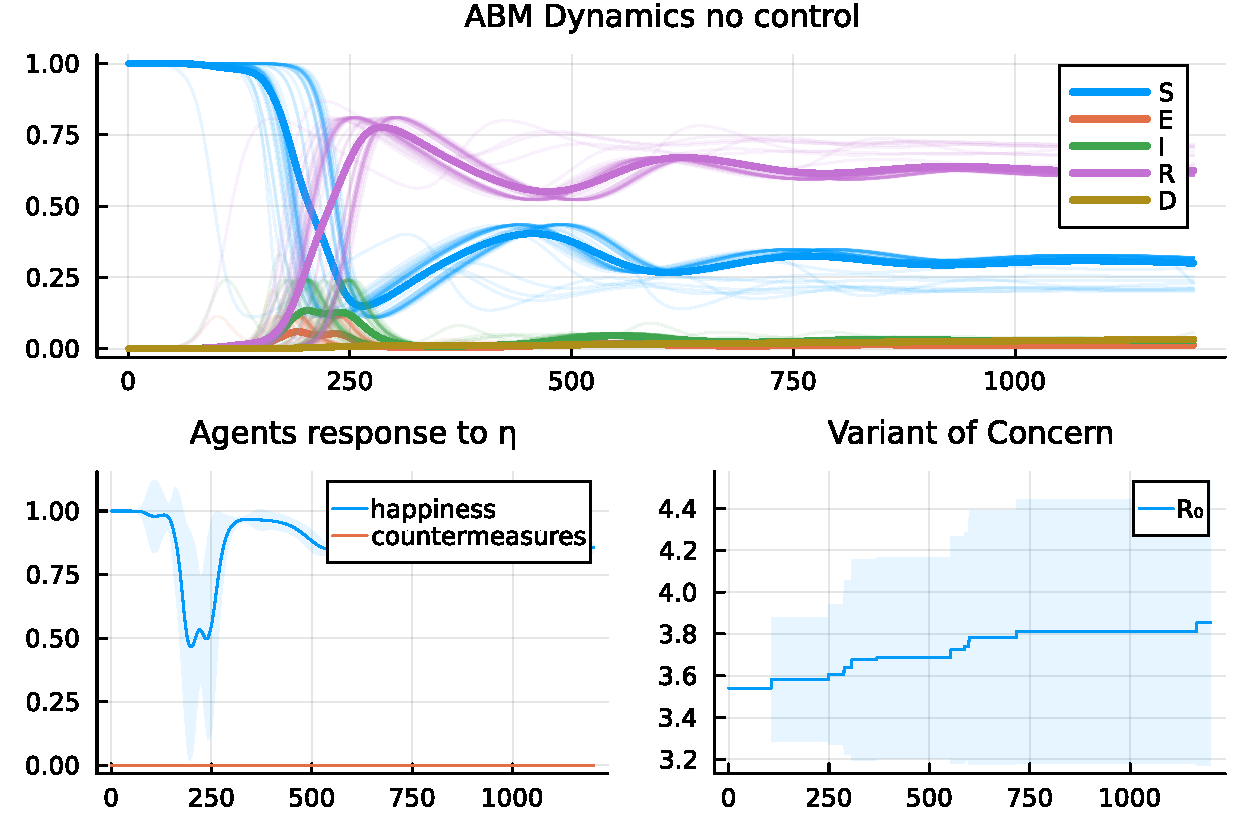
\includegraphics[width=\textwidth]{img/SocialNetworkABM_NO_CONTROL.pdf}
	\captionof{figure}{Grafico cumulativo del risultato del modello senza intervento del controllore}
	\label{fig:abm_no_intervent}
\end{minipage}

Complessivamente pero' l'andamento e' ovviamente similare ad un andamento standard di un modello 
SEIR, con qualche variazione dipendente dai fattori di stocasticita' del modello che pero'
in questo caso non risultano troppo presenti, che vengono messi in evidenza con le curve del modello 
meno marcate, che rappresentano i percorsi "meno battuti" della simulazione.

Come e' possibile notare, il numero di individui suscettibili crolla drasticamente
per via della diffusione rapida e simil esponenziale che ha il virus. Questa viene emulata
dall'altrettanto rapida crescita di individui guariti (recovered) che pero', per via
di come e' stato definita la condizione di guariti, non sono immuni alle varianti del virus. 
Queste proprieta' contribuiscono ad un andamento ciclico delle curve, in particolar modo 
di quelle \emph{E, I, R}. La curva associata al compartimento \emph{S} ha un suo andamento
ciclico seppur molto sottile; questa sottigliezza e' dovuta all'assenza di misure di 
controllo all'interno del sistema.

Si puo' infine notare come la curva associata all'andamento degli individui
nella classe \emph{D} abbia una crescita lineare, seppur non troppo evidente.

A seguire si puo' osservare come la curva associata alla variabile di happiness del modello,
valore che serve per bilanciare la durezza delle misure di controllo per evitare 
di cadere in un ciclo funzionale ma insostenibile, mostra un comportamento alquanto bizzarro.
Questo e' dovuto principalmente a come viene definita la funzione di controllo della felicita' 
la quale essendo dominata principalmente da due fattori, $\eta$ ovvero le contromisure applicate
da un controllore e dalla proporzione tra il numero di individui nelle categorie \textbf{S, R} e 
gli individui nelle categorie \textbf{I, D} si arriva velocemente a comprenderne il funzionamento.
Si osserva inoltre che la curva tende ad un \emph{plateau} passato il periodo della "prima ondata". 

Questo comportamento e' irrealistico e associato alla definizione che e' stata fatta della 
funzione \textbf{happiness!}. Tuttavia anche se il comportamento di questa curva non e' 
completamente realistico, si puo' comunque utilizzare per mantenere sotto controllo le contromisure $\eta$.

Infine si nota come, seppur la definizione della funzione associata alla creazione di una
nuova \emph{Variant of Concern (VOC)} \ref{fig:voc} sia semplicistica e irrealistica, 
il grafico mostra come su un periodo di circa 3 anni, associabile alla durata del periodo covid, 
le voc sono al piu' una decina (ogni picco o depressione e' una voc). 

\begin{minipage}{\linewidth}
	\centering
	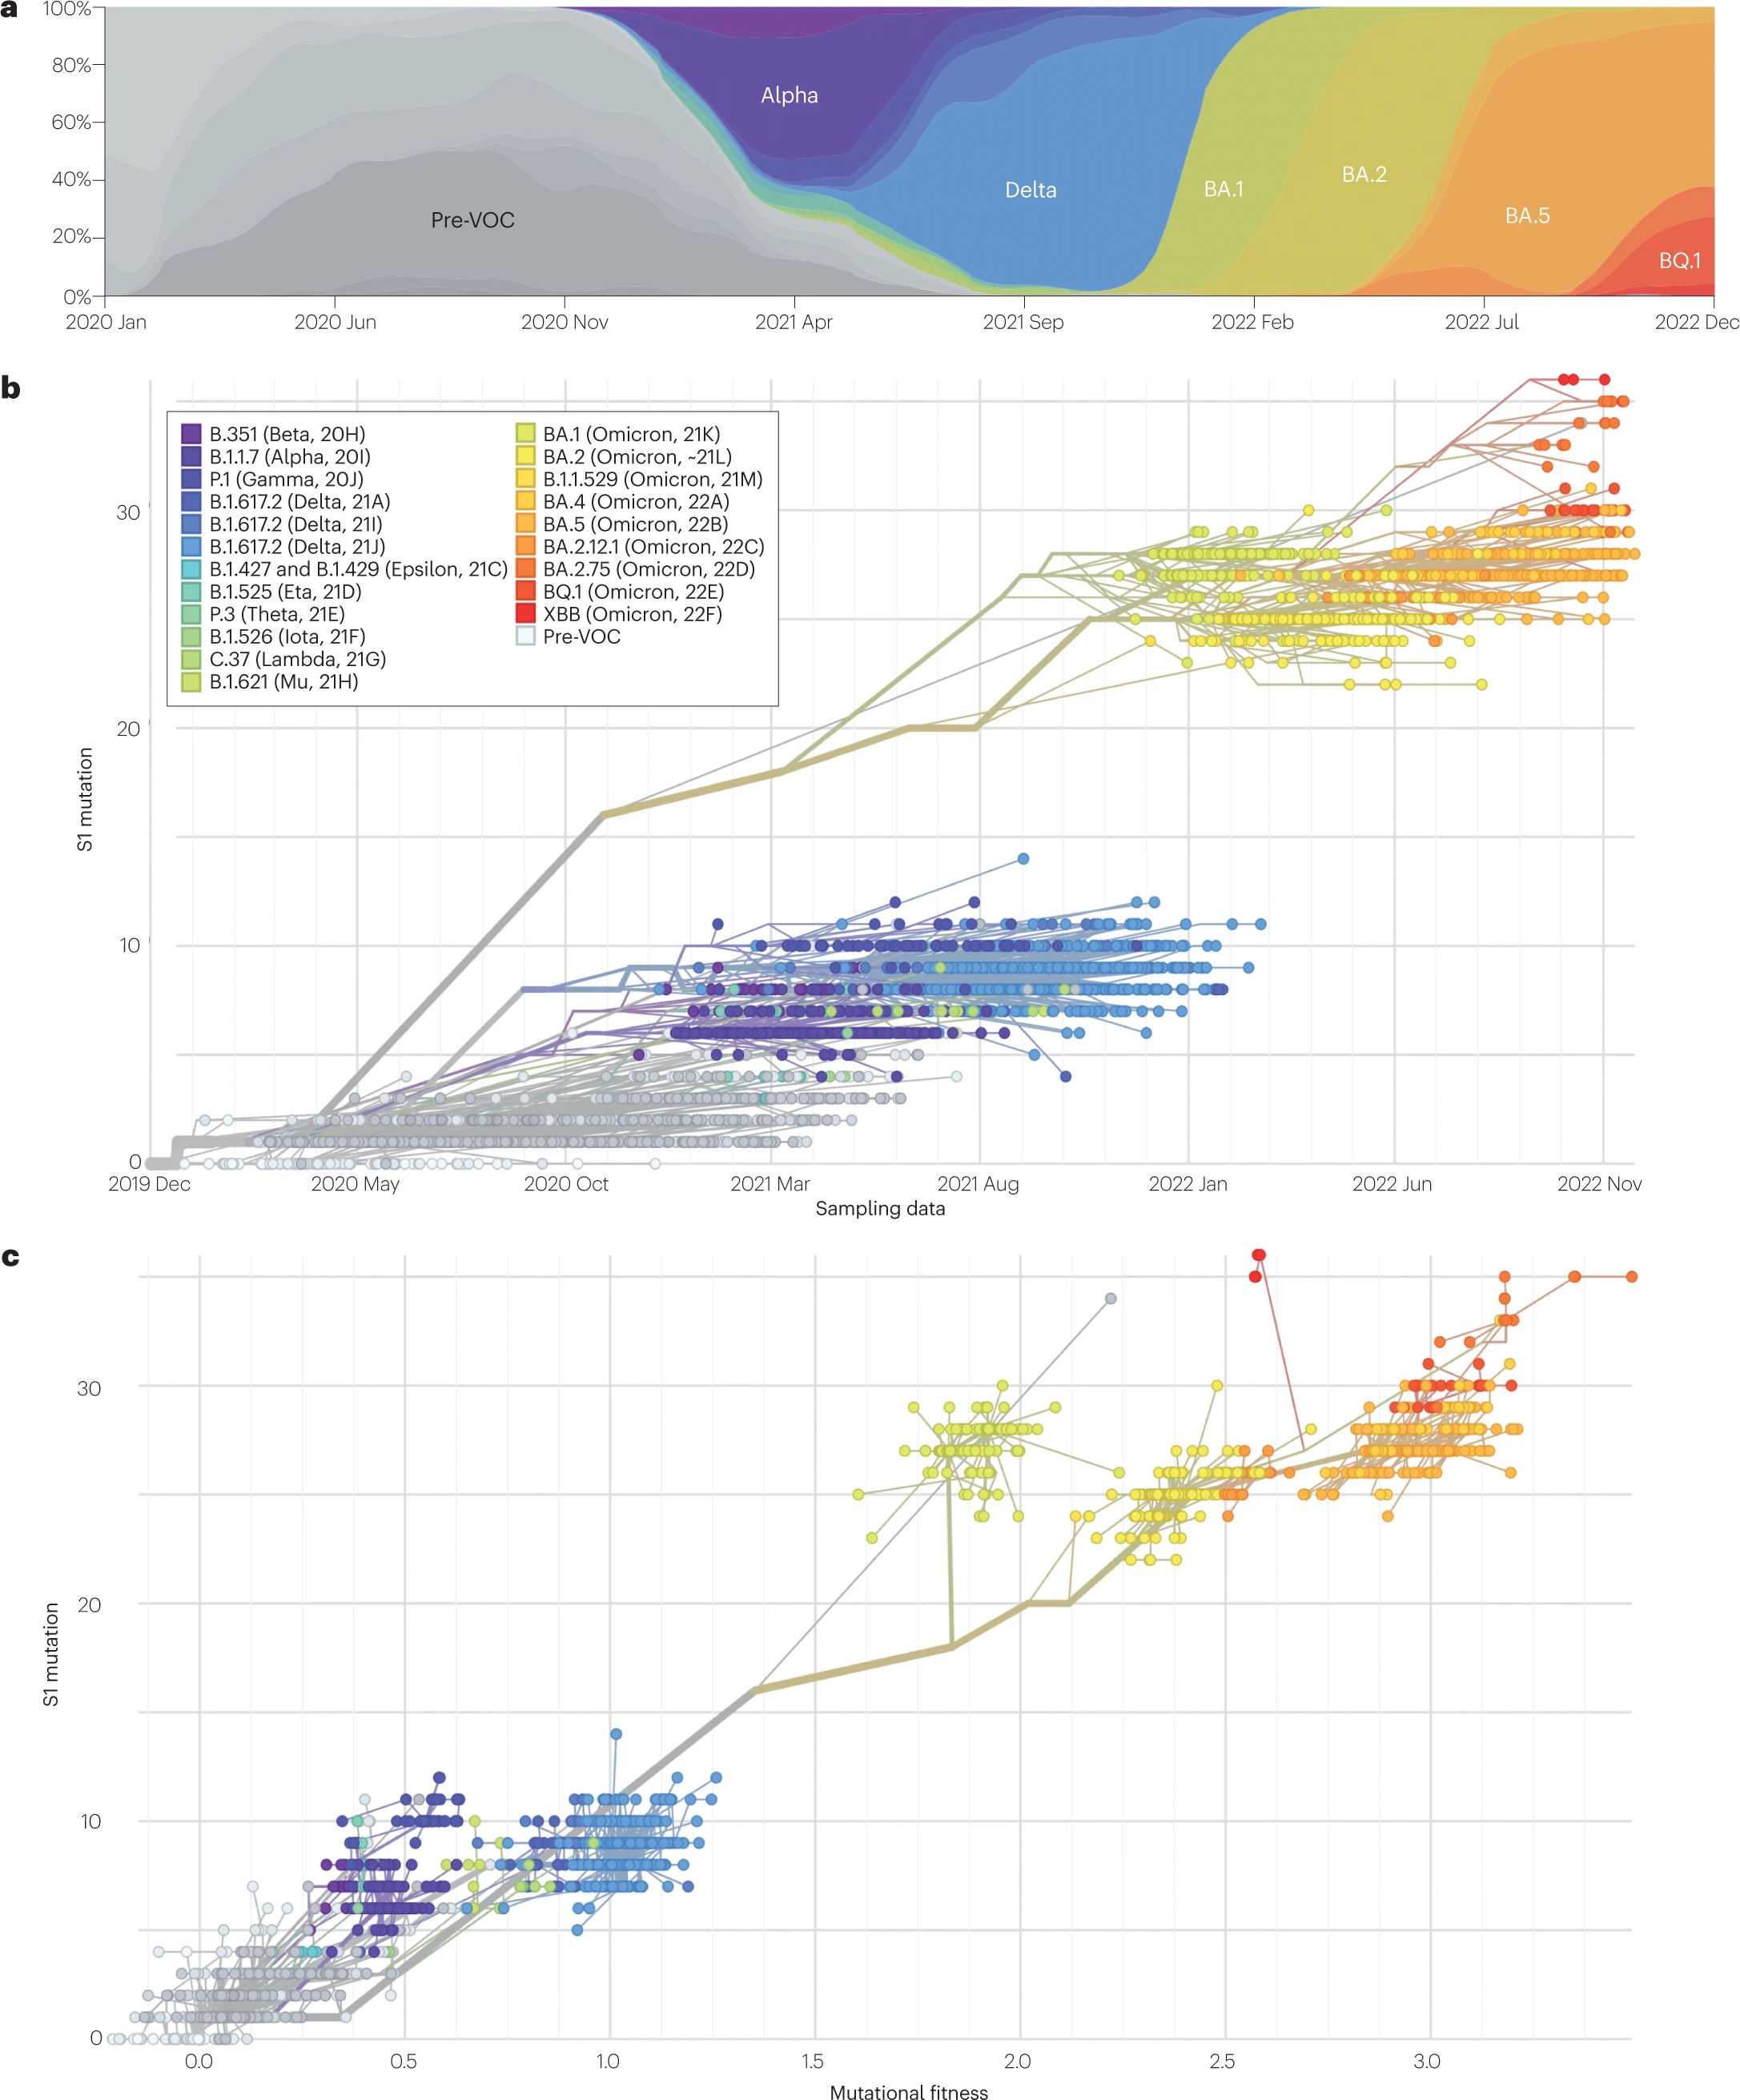
\includegraphics[width=\textwidth, height=\textheight]{img/41579_2023_878_Fig3_HTML.png}
	\captionof{figure}{Grafico delle mutazioni casuali del virus SARS-COV2 preso dall'articolo \cite{Markov2023}}
	\label{fig:covid_mutation}
\end{minipage}

Si nota come le voc scoperte del covid siano una quantita' pressoche' similare seppur con una 
distribuzione all'interno della linea temporale differente. Tuttavia il comportamento semplicistico 
applicato nel modello sembra essere una buona approssimazione del comportamento reale del virus.

\subsubsection*{Grafico con intervento non farmaceutico}

Il seguente grafico \ref{fig:abm_intervent} mostra l'andamento delle curve del modello
quando questo viene eseguito tramite l'applicazione di una qualche tipologia di intervento non farmaceutico. 
Questo andamento tuttavia e' mostrato in maniera cumulativa rispetto all'andamento dei singoli agenti, il quale puo' avere comportamentei 
differenti in base a se appare o meno una variante, come specificato in figura \ref{fig:voc}, oppure 
dipendentemente dal tipo di contromisure applicate. 

\begin{minipage}{\linewidth}
	\centering
	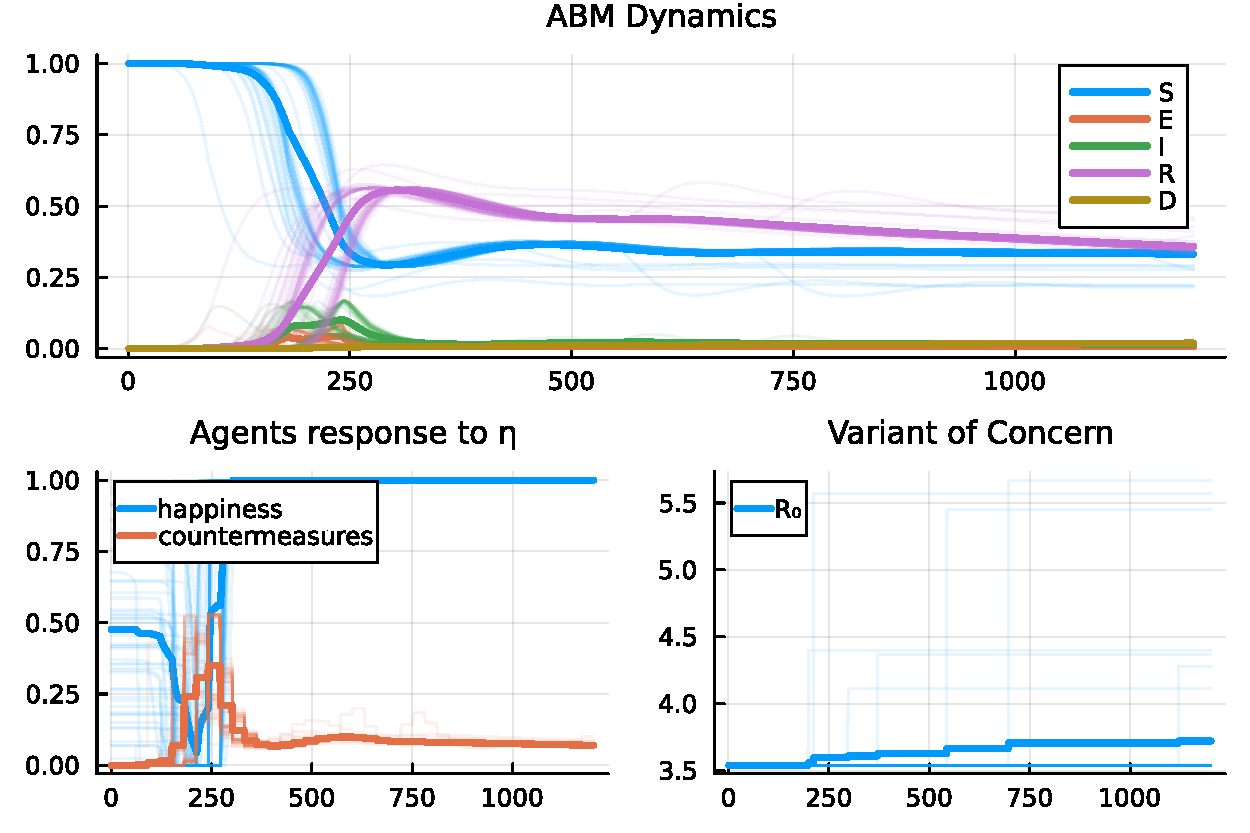
\includegraphics[width=\textwidth]{img/SocialNetworkABM_CONTROL.pdf}
	\captionof{figure}{Grafico cumulativo del risultato del modello con intervento del controllore}
	\label{fig:abm_intervent}
\end{minipage}

Si puo' notare come le varie curve rappresentate siano molto piu' accentuate mostrando percorsi differenti 
ma comunque simili nell'andamento generale. La curva associata alla felicita' e' altalenante e segue generalmente
l'andamento delle contromisure applicate dal controllore alla popolazione. In questo caso vi sono curve
molto differenti che mostrano comportamenti altrettanto differenti, ma in generale il comportamento e' 
relativamente contenuto e non eccessivo. 

Altro dato interessante e' il numero di VOC che pare essere diminuito rispetto al modello senza intervento.
Questo dipende generalmente dal comportamento delle contromisure. Infatti queste quando vengono applicate, 
oltre a influenzare il parametro \textbf{happiness}, vanno ad influenzare anche la matrice di flusso \ref{fig:migration matrix}
andando a ridurne i valori presenti. Questo fa si che oltre a dilazionare la diffusione della pandemia, andando 
ad applicare involontariamente delle contromisure simil lockdown e smart working (per prevenire il forte afflusso di individui),
va anche a dilazionare il comportamento della funzione che si occupa di generare una VOC \ref{fig:voc}. 

Questa infatti puo' attivarse sse nel nodo sono presenti individui infetti, in quanto non e' stata modellata la 
possibilita' che spontaneamente una nuova variante arrivi in un nuovo nodo senza un veicolo umano. Percio' 
applicare delle contromisure permette anche a contenere la diffusione di VOC nella popolazione osservata.

\subsubsection*{Grafico con intervento farmaceutico}
Il seguente grafico \ref{fig:abm_vaccine} mostra l'andamento delle curve del modello
quando questo viene eseguito tramite l'applicazione di una qualche tipologia di intervento farmaceutico. 
Questo andamento tuttavia e' mostrato in maniera cumulativa rispetto all'andamento dei singoli agenti, 
il quale puo' avere comportamenti differenti in base a se appare o meno una variante, 
come specificato in figura \ref{fig:voc}, oppure dipendentemente dal tipo di contromisure applicate.

\begin{minipage}{\linewidth}
	\centering
	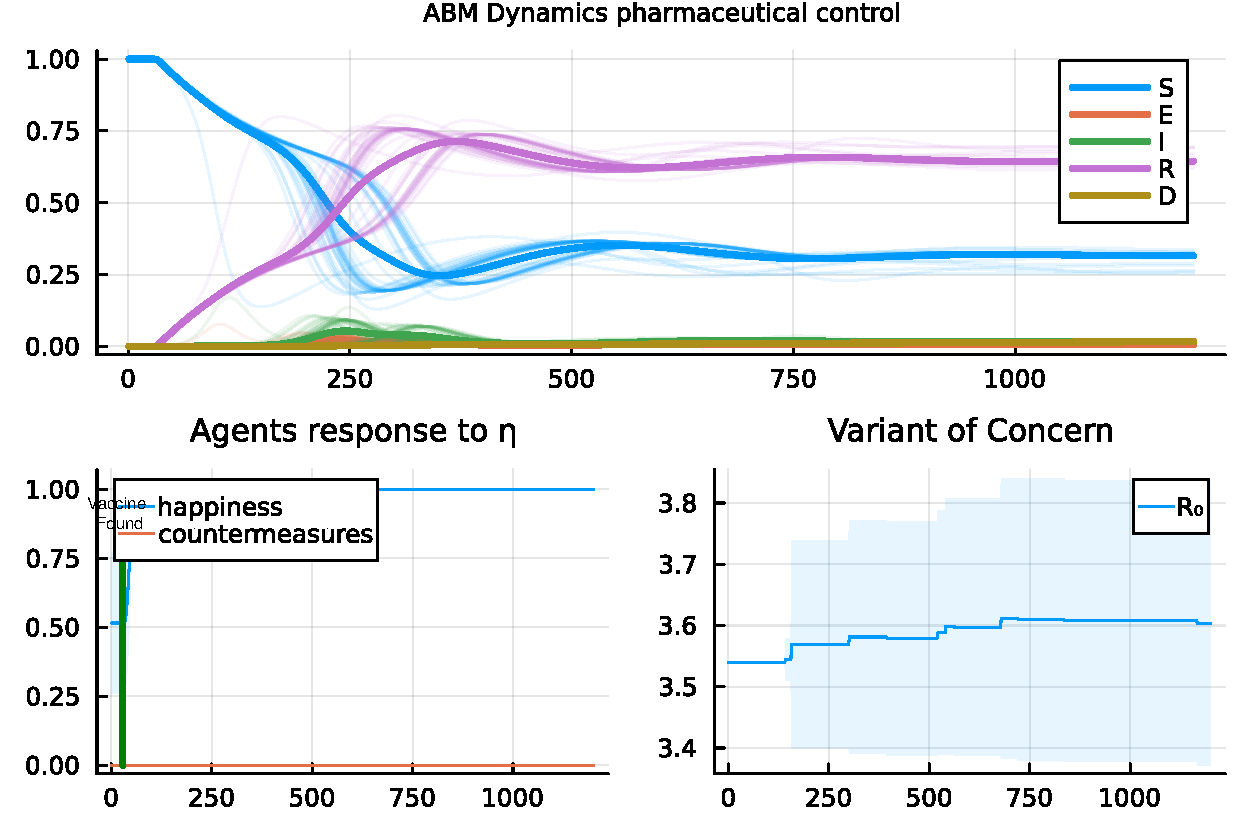
\includegraphics[width=\textwidth]{img/SocialNetworkABM_VACCINE.pdf}
	\captionof{figure}{Grafico cumulativo del risultato del modello con intervento del controllore tramite vaccino}
	\label{fig:abm_vaccine}
\end{minipage}

Come accennato con il grafico in figura \ref{fig:abm_intervent} il grafico relativo al cambiamento 
del valore $R_0$, quindi indice di quante varianti compaiono in un determinato periodo di tempo, e' 
ulteriormente influenzato dalla presenza di un vaccino, in quanto rende la popolazione immune per
un determinato periodo di tempo al virus, rendendo quest'ultimo meno influente e meno incline alla
creazione di nuove varianti, le quali, una volta create paiono essere di media meno pericolose, avendo un 
valore $R_0$ medio meno alto rispetto a quelle dei grafici \ref{fig:abm_intervent} e \ref{fig:abm_no_intervent}.

Questo grafico tuttavia puo' cambiare drasticamente in base a quando un vaccino viene effettivamente scoperto e 
rilasciato sul mercato come metodo per contrastare un'epidemia.

\subsubsection*{Grafico con intervento farmaceutico e non farmaceutico}
Il seguente grafico \ref{fig:abm_all} mostra l'andamento delle curve del modello
quando questo viene eseguito tramite l'applicazione di una qualche tipologia di intervento farmaceutico. 
Questo andamento tuttavia e' mostrato in maniera cumulativa rispetto all'andamento dei singoli agenti, 
il quale puo' avere comportamenti differenti in base a se appare o meno una variante, 
come specificato in figura \ref{fig:voc}, oppure dipendentemente dal tipo di contromisure applicate.

\begin{minipage}{\linewidth}
	\centering
	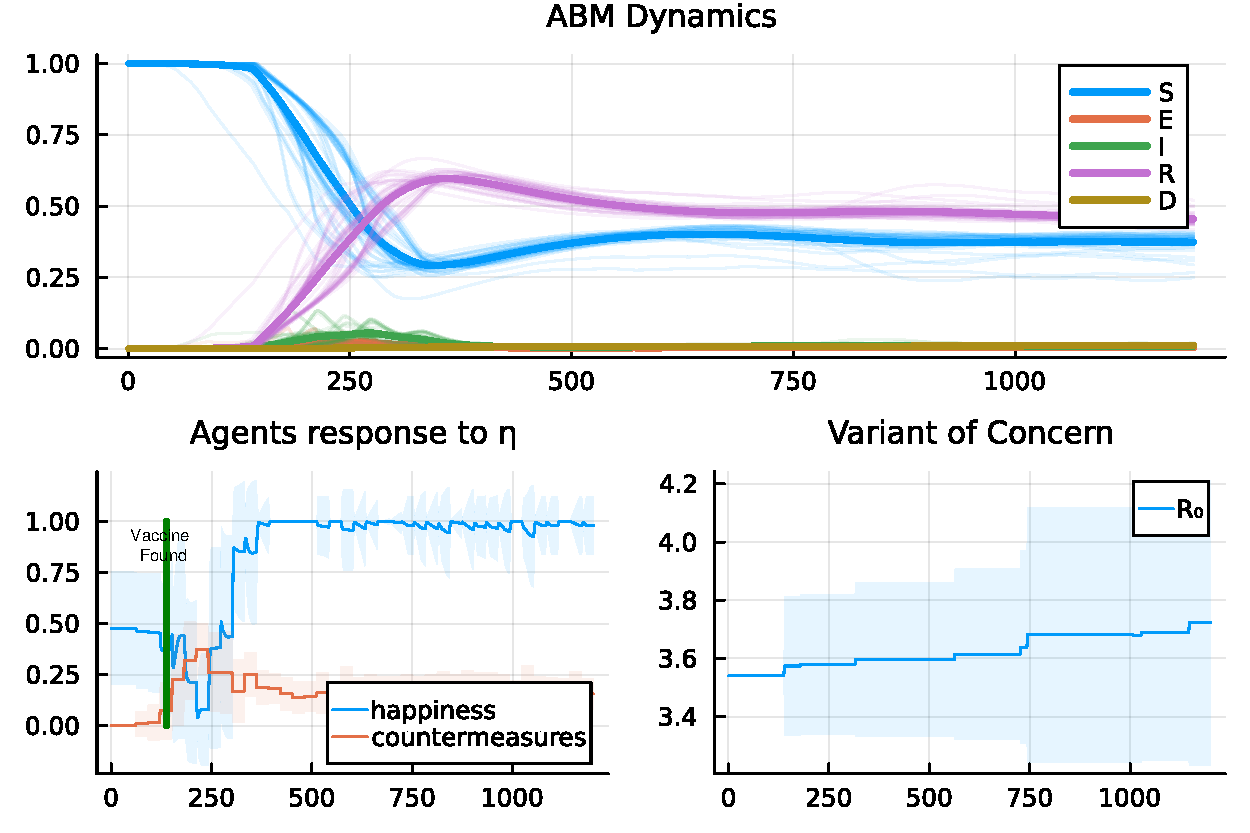
\includegraphics[width=\textwidth]{img/SocialNetworkABM_ALL.pdf}
	\captionof{figure}{Grafico cumulativo del risultato del modello con intervento del controllore tramite vaccino e metodi di prevenzione non farmaceutici}
	\label{fig:abm_all}
\end{minipage}

In questo caso viene mostrata l'andamento delle curve tenendo in considerazione l'utilizzo di ogni mezzo
per prevenire e contrastare l'epidemia. L'uitilizzo combinato di mezzi farmaceutici e non permettono 
si appiattire notevolmente la curva di infetti andando a creare velocemente un immunita' di gruppo 
che rende la popolazione meno suscettibile alle varianti. Questo inoltre fa si che la \emph{happiness} media
del modello sia generalmente piu' alta anche quando vengono applicate delle contromisure che vanno ad 
intaccare la felicita' della popolazione (ad esempio un lockdown). 

Queste contromisure non farmaceutiche sono in genere meno stringenti e meno prolungate, permettendo quindi
alla popolazione di non avere un calo drastico della happiness generale come in figura \ref{fig:abm_intervent}.
Tuttavia dipendono fortemente da quando le contromisure farmaceutiche (il vaccino) vengono applicate
e con che efficacia questo riesce ad entrare in circolazione. 

Tuttavia questo dimostra come l'utilizzo di un vaccino a priori sia un metodo molto efficace per contrastare
una epidemia, e che ovviamente l'efficacia di questo dipenda molto e soprattutto da quando viene applicato 
alla popolazione. Successivamente si puo' notare come le misure non farmaceutiche di prevenzione e contrasto
dell'epidemia sono un mezzo efficace per controllare la diffusione dell'infezione, ma queste hanno un costo 
in termini sia di generale qualita' della vita, che anche economico, non indifferente come mostrato dai grafici 
precedenti e dall'esperienza diretta che si e' avuto con la pandemia da COVID-19. 